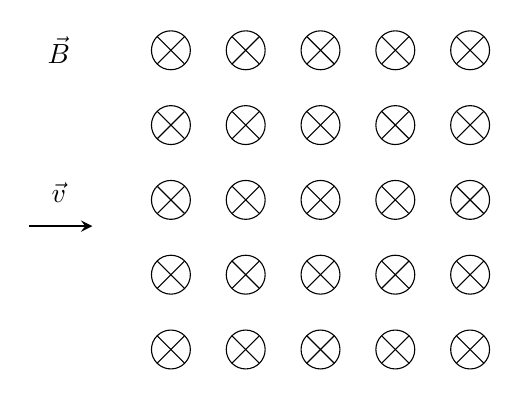
\begin{tikzpicture}[x=0.95cm,y=0.95cm]
  % 5x5 grid of "B into page" symbols (circle with diagonal cross)
  \foreach \r in {0,...,4}{
    \foreach \c in {0,...,4}{
      \begin{scope}[shift={(\c,-\r)}]
        \draw (0,0) circle (0.26);
        \draw (-0.18,-0.18) -- (0.18,0.18);
        \draw (-0.18,0.18) -- (0.18,-0.18);
      \end{scope}
    }
  }
  \node at (-1.5,0) {$\vec{B}$};
  \node at (-1.5,-1.9) {$\vec{v}$};
  \draw[->,>=stealth,thick] (-1.9,-2.35) -- (-1.05,-2.35);
\end{tikzpicture}
